% figures/warp-vs-cta-tiles.tex
% Physical tile shapes: the 32-thread warp tile, the 128-thread CTA
% tile, and the 512-thread split tile.
\documentclass[tikz,border=10pt]{standalone}
% figures/common-preamble.tex
% Shared setup for the TikZ documentation figures. Colors mirror the
% palette in scripts/render_docs_diagrams.py so both atlases match.
\usepackage[T1]{fontenc}
\usepackage{lmodern}
\usepackage{tikz}
\usepackage{pgfplots}
\pgfplotsset{compat=1.18}
\usetikzlibrary{arrows.meta}
\usetikzlibrary{backgrounds}
\usetikzlibrary{calc}
\usetikzlibrary{decorations.pathreplacing}
\usetikzlibrary{fit}
\usetikzlibrary{positioning}

\definecolor{swcanvas}{HTML}{FFFDF8}
\definecolor{swpanel}{HTML}{F5F3ED}
\definecolor{swink}{HTML}{17212B}
\definecolor{swmuted}{HTML}{4B5563}
\definecolor{swline}{HTML}{59636E}
\definecolor{swblue}{HTML}{00689D}
\definecolor{swbluefill}{HTML}{DCEFFD}
\definecolor{swpurple}{HTML}{8E4775}
\definecolor{swpurplefill}{HTML}{F7E2EF}
\definecolor{sworange}{HTML}{A94500}
\definecolor{sworangefill}{HTML}{FCE5DC}
\definecolor{swgreen}{HTML}{00664B}
\definecolor{swgreenfill}{HTML}{DDF4EB}
\definecolor{swgrayfill}{HTML}{EEF0F2}

\pagecolor{swcanvas}
\AtBeginDocument{\color{swink}}

\tikzset{
  swcell/.style={
    draw, minimum width=0.46cm, minimum height=0.46cm, inner sep=0pt,
    line width=0.7pt, rounded corners=1pt},
  swbox/.style={
    draw=swline, fill=swpanel, rounded corners=6pt, line width=0.9pt},
  swarrow/.style={-{Stealth[length=6pt]}, draw=swline, line width=1pt},
  swtag/.style={
    draw, rounded corners=8pt, line width=0.9pt,
    font=\bfseries\scriptsize, inner xsep=8pt, inner ysep=4pt},
  swtitle/.style={anchor=west, font=\Large\bfseries, text=swink},
  swsubtitle/.style={anchor=west, font=\small, text=swmuted},
  swcode/.style={font=\small\ttfamily, text=swink},
  every picture/.style={line cap=round},
}

\begin{document}
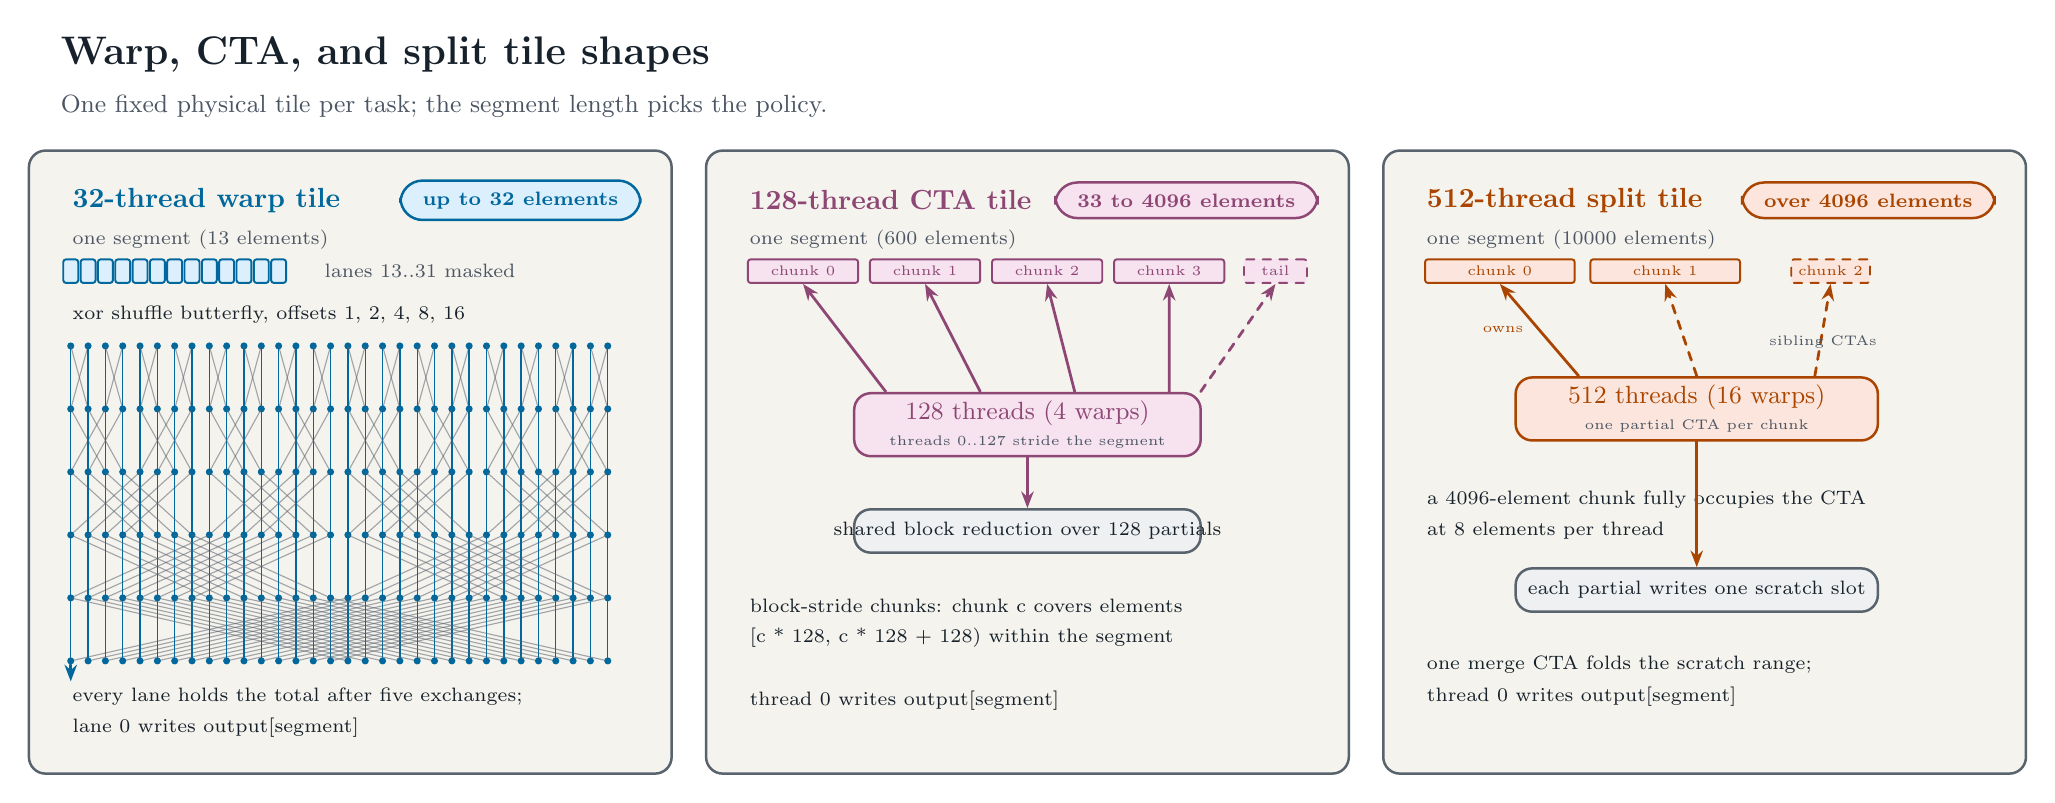
\begin{tikzpicture}[x=1cm, y=1cm]

% Header.
\node[swtitle] at (0, 1.3) {Warp, CTA, and split tile shapes};
\node[swsubtitle] at (0, 0.65)
  {One fixed physical tile per task; the segment length picks the
   policy.};

% ---------------------------------------------------------------- warp
\node[swbox, fit={(0, -7.55) (7.6, -0.2)}, inner sep=8pt] {};
\node[anchor=west, font=\bfseries, text=swblue] at (0.15, -0.55)
  {32-thread warp tile};
\node[swtag, draw=swblue, fill=swbluefill, text=swblue, anchor=east]
  at (7.5, -0.55) {up to 32 elements};

% One short segment feeding the warp lanes.
\node[anchor=west, font=\scriptsize, text=swmuted] at (0.15, -1.05)
  {one segment (13 elements)};
\foreach \i in {0,...,12} {
  \node[swcell, minimum width=0.19cm, minimum height=0.3cm,
        fill=swbluefill, draw=swblue] at (0.25 + \i * 0.22, -1.45) {};
}
\node[anchor=west, font=\scriptsize, text=swmuted] at (3.35, -1.45)
  {lanes 13..31 masked};

% Xor shuffle butterfly: every stage combines lane l with lane l xor
% offset, so all 32 lanes stay live and end holding the total.
\node[anchor=west, font=\scriptsize, text=swink] at (0.15, -2.0)
  {xor shuffle butterfly, offsets 1, 2, 4, 8, 16};
\foreach \l in {0,...,31} {
  \fill[swblue] ({0.25 + \l * 0.22}, -2.4) circle (0.045);
}
\foreach \s/\o in {1/1, 2/2, 3/4, 4/8, 5/16} {
  \foreach \l in {0,...,31} {
    \pgfmathtruncatemacro{\partner}{
      mod(floor(\l / \o), 2) == 0 ? \l + \o : \l - \o}
    \draw[swline, line width=0.4pt, opacity=0.55]
      ({0.25 + \partner * 0.22}, {-2.4 - (\s - 1) * 0.8})
      -- ({0.25 + \l * 0.22}, {-2.4 - \s * 0.8});
    \draw[swblue, line width=0.5pt]
      ({0.25 + \l * 0.22}, {-2.4 - (\s - 1) * 0.8})
      -- ({0.25 + \l * 0.22}, {-2.4 - \s * 0.8});
    \fill[swblue] ({0.25 + \l * 0.22}, {-2.4 - \s * 0.8})
      circle (0.045);
  }
}
\node[anchor=west, font=\scriptsize, text=swink] at (0.15, -6.85)
  {every lane holds the total after five exchanges;};
\node[anchor=west, font=\scriptsize, text=swink] at (0.15, -7.25)
  {lane 0 writes output[segment]};
\draw[swarrow, draw=swblue] (0.25, -6.45) -- (0.25, -6.66);

% ----------------------------------------------------------------- cta
\node[swbox, fit={(8.6, -7.55) (16.2, -0.2)}, inner sep=8pt] {};
\node[anchor=west, font=\bfseries, text=swpurple] at (8.75, -0.55)
  {128-thread CTA tile};
\node[swtag, draw=swpurple, fill=swpurplefill, text=swpurple,
      anchor=east] at (16.1, -0.55) {33 to 4096 elements};

% One longer segment split into block-stride chunks.
\node[anchor=west, font=\scriptsize, text=swmuted] at (8.75, -1.05)
  {one segment (600 elements)};
\foreach \c/\lab in {0/{chunk 0}, 1/{chunk 1}, 2/{chunk 2}, 3/{chunk 3}} {
  \node[swcell, minimum width=1.4cm, minimum height=0.3cm,
        fill=swpurplefill, draw=swpurple]
    (chunk\c) at (9.55 + \c * 1.55, -1.45) {};
  \node[font=\tiny, text=swpurple] at (9.55 + \c * 1.55, -1.45) {\lab};
}
\node[swcell, minimum width=0.8cm, minimum height=0.3cm,
      fill=swpurplefill, draw=swpurple, dashed]
  (chunktail) at (15.55, -1.45) {};
\node[font=\tiny, text=swpurple] at (15.55, -1.45) {tail};

% The thread block revisits chunks in a block-stride loop.
\node[swbox, fill=swpurplefill, draw=swpurple,
      minimum width=4.4cm, minimum height=0.8cm]
  (ctablock) at (12.4, -3.4) {};
\node[font=\small, text=swpurple] at (12.4, -3.25)
  {128 threads (4 warps)};
\node[font=\tiny, text=swmuted] at (12.4, -3.62)
  {threads 0..127 stride the segment};
\foreach \c in {0,...,3} {
  \draw[swarrow, draw=swpurple]
    (10.6 + \c * 1.2, -2.98) -- (chunk\c.south);
}
\draw[swarrow, draw=swpurple, dashed] (14.6, -2.98) -- (chunktail.south);

% Block reduction and the single writer.
\node[swbox, fill=swgrayfill, minimum width=4.4cm,
      minimum height=0.55cm] (blockred) at (12.4, -4.75) {};
\node[font=\scriptsize, text=swink] at (12.4, -4.75)
  {shared block reduction over 128 partials};
\draw[swarrow, draw=swpurple] (ctablock.south) -- (blockred.north);
\node[anchor=west, font=\scriptsize, text=swink] at (8.75, -5.7)
  {block-stride chunks: chunk c covers elements};
\node[anchor=west, font=\scriptsize, text=swink] at (8.75, -6.1)
  {[c * 128, c * 128 + 128) within the segment};
\node[anchor=west, font=\scriptsize, text=swink] at (8.75, -6.9)
  {thread 0 writes output[segment]};

% --------------------------------------------------------------- split
\node[swbox, fit={(17.2, -7.55) (24.8, -0.2)}, inner sep=8pt] {};
\node[anchor=west, font=\bfseries, text=sworange] at (17.35, -0.55)
  {512-thread split tile};
\node[swtag, draw=sworange, fill=sworangefill, text=sworange,
      anchor=east] at (24.7, -0.55) {over 4096 elements};

% One huge segment decomposed into ordered 4096-element chunks.
\node[anchor=west, font=\scriptsize, text=swmuted] at (17.35, -1.05)
  {one segment (10000 elements)};
\foreach \c/\lab in {0/{chunk 0}, 1/{chunk 1}} {
  \node[swcell, minimum width=1.9cm, minimum height=0.3cm,
        fill=sworangefill, draw=sworange]
    (split\c) at (18.4 + \c * 2.1, -1.45) {};
  \node[font=\tiny, text=sworange] at (18.4 + \c * 2.1, -1.45) {\lab};
}
\node[swcell, minimum width=1.0cm, minimum height=0.3cm,
      fill=sworangefill, draw=sworange, dashed]
  (split2) at (22.6, -1.45) {};
\node[font=\tiny, text=sworange] at (22.6, -1.45) {chunk 2};

% One partial CTA owns exactly one chunk.
\node[swbox, fill=sworangefill, draw=sworange,
      minimum width=4.6cm, minimum height=0.8cm]
  (splitcta) at (20.9, -3.2) {};
\node[font=\small, text=sworange] at (20.9, -3.05)
  {512 threads (16 warps)};
\node[font=\tiny, text=swmuted] at (20.9, -3.42)
  {one partial CTA per chunk};
\draw[swarrow, draw=sworange] (19.4, -2.78) -- (split0.south)
  node[midway, left=2pt, font=\tiny, text=sworange] {owns};
\draw[swarrow, draw=sworange, dashed] (20.9, -2.78) -- (split1.south);
\draw[swarrow, draw=sworange, dashed] (22.4, -2.78) -- (split2.south);
\node[font=\tiny, text=swmuted, anchor=west] at (21.7, -2.35)
  {sibling CTAs};
\node[anchor=west, font=\scriptsize, text=swink] at (17.35, -4.35)
  {a 4096-element chunk fully occupies the CTA};
\node[anchor=west, font=\scriptsize, text=swink] at (17.35, -4.75)
  {at 8 elements per thread};

% Partials write scratch; one merge folds it into the output.
\node[swbox, fill=swgrayfill, minimum width=4.6cm,
      minimum height=0.55cm] (scratch) at (20.9, -5.5) {};
\node[font=\scriptsize, text=swink] at (20.9, -5.5)
  {each partial writes one scratch slot};
\draw[swarrow, draw=sworange] (splitcta.south) -- (scratch.north);
\node[anchor=west, font=\scriptsize, text=swink] at (17.35, -6.45)
  {one merge CTA folds the scratch range;};
\node[anchor=west, font=\scriptsize, text=swink] at (17.35, -6.85)
  {thread 0 writes output[segment]};

\end{tikzpicture}
\end{document}
